\section{Rates in the unselective regime}
\label{app:dephasing_unselective}
\subsection{Dephasing rates}
This subsection benchmarks the analytical dephasing rates in Eq.~\eqref{eq:Gamma_phi_total_unselective} against numerical simulations. The numerical reference rate for
\(\gamma_{b\uparrow}^{\mathrm{un}}+\gamma_{c\phi}^{\mathrm{un}}\) is extracted using the procedure in App.~\ref{app:dephasing_numerics}, with the flux-noise drive set to \(\delta\Phi(t)=0\).

In the large-detuning regime, the reference rate is well captured by the analytical approximation in Fig.~\ref{fig:relaxation_excitation_plot}(a):
\begin{align}
&\gamma_{b\uparrow}^{\mathrm{un}}+\gamma_{c\phi}^{\mathrm{un}}\\
&=
\frac{\gamma_{b\downarrow}}{16}\left(\frac{\Delta_{bd}}{K}\right)^2
\left(1-\frac{2\Delta_{bd}}{K}\right)
+\frac{\gamma_{b\downarrow}}{2}\left(\frac{g}{\Delta_{bc}}\right)^4\frac{K}{\Delta_{bd}} .
\label{eq:gamma_unselective_approx}
\end{align}

In this limit, dephasing is dominated by photon-shot noise from heating, i.e., \(\gamma_{b\uparrow}^{\mathrm{un}}\), while \(\gamma_{c\phi}^{\mathrm{un}}\) is parametrically suppressed at large detuning, consistent with Eq.~\eqref{eq:gamma_unselective_approx}.

As the detuning decreases, the numerical and analytical results deviate because Eq.~\eqref{eq:gamma_unselective_approx} assumes \(|\Delta_{bd}/\chi|\gg 1\) (here \(\chi/2\pi \simeq -2\,\mathrm{MHz}\)). In this regime, the total dephasing rate increases and \(\gamma_{c\phi}^{\mathrm{un}}\) becomes the dominant contribution.

Finally, the flux-noise-induced depolarization rate is benchmarked numerically against
\begin{equation}
\gamma_{b\uparrow}^{1/f,\mathrm{un}}=
\left(\frac{\partial\omega_b}{\partial\Phi}\right)^2\frac{S_0^2}{4K}.
\end{equation}
The simulation is initialized in the Floquet ground state \(|\phi_{g0}(0)\rangle\), and the excitation rate is extracted by fitting the average overlap
\(\mathrm{Tr}\!\left[\rho\,|\phi_{g0}(0)\rangle\langle\phi_{g0}(0)|\right]\) to \(\frac{1}{2}\!\left(1-e^{-2\gamma_{b\uparrow}^{1/f,\mathrm{un}} t}\right)\).
Sweeping the noise amplitude \(S_0\) yields a quadratic scaling, and the numerical results follow the analytical prediction (black dashed line) closely [Fig.~\ref{fig:relaxation_excitation_plot}(b)]. The small error bars in the figure indicate statistical convergence for the chosen ensemble size ($N=100$ trajectories).

\begin{figure}
    \centering
    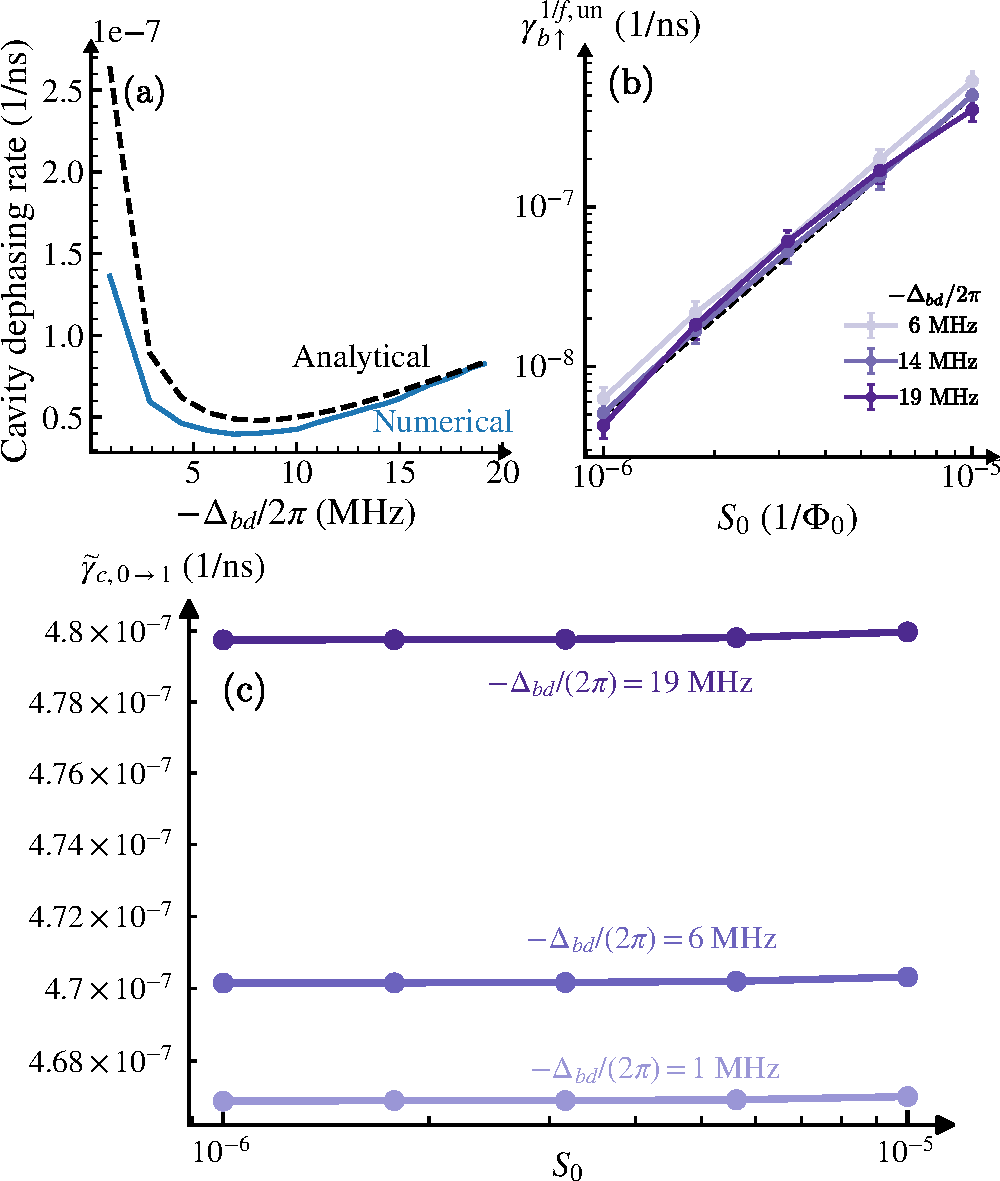
\includegraphics[width=\linewidth]{Appendix/relaxation_excitation_plot.pdf}
    \caption{Numerical validation of rates in the unselective regime.
(a) Reference dephasing rate \(\gamma_{b\uparrow}^{\mathrm{un}}+\gamma_{c\phi}^{\mathrm{un}}\) extracted from the procedure in App.~\ref{app:dephasing_numerics} with \(\delta\Phi(t)=0\), compared with the analytical approximation in Eq.~\eqref{eq:gamma_unselective_approx}.
(b) Flux-noise-induced depolarization rate \(\gamma_{b\uparrow}^{1/f,\mathrm{un}}\) versus noise amplitude \(S_0\). The quadratic scaling in \(S_0\) and agreement with \(\gamma_{b\uparrow}^{1/f,\mathrm{un}}=\left(\frac{\partial\omega_b}{\partial\Phi}\right)^2\frac{S_0^2}{4K}\) (black dashed line) are observed.
(c) Cavity decay rate with sweet-spot drive.}
    \label{fig:relaxation_excitation_plot}
\end{figure}

\subsection{Decay rates}
This subsection shows that the cavity decay rate is only weakly affected by the drive. For the parameters used to generate Fig.~\ref{fig:total_rate}, the undriven decay rate is \(4.75\times10^{-7}\,\mathrm{ns}^{-1}\). Under drive, the decay rate remains nearly unchanged, as shown in Fig.~\ref{fig:relaxation_excitation_plot}(c).
% We observe quantitative discrepancies between theoretical expectations and our simulated rates for both transmon excitation and cavity dephasing. Using the analytical model, the expected $|00\rangle \to |10\rangle$ heating rate is roughly $\gamma_{00\to 10} \approx 2.0 \times 10^{-6} \text{ ns}^{-1}$, calculated via the relation $(A/\Delta_{bd})^2 (\frac{\partial \omega_b}{\partial \Phi} S_0)^2 / (\Delta_{bd}/2\pi)$. However, the value extracted from the simulation fit is notably higher, at $3.5 \times 10^{-6} \text{ ns}^{-1}$. As expected from both theory and simulation, heating out of the 1-photon state ($|01\rangle \to |11\rangle$) is negligible; given $\Delta_{bd} \approx 0.9 \text{ MHz}$ and $\chi \approx 2.1 \text{ MHz}$, this rate is theoretically suppressed by a factor of ${\sim}27$ due to its scaling with $(\Delta_{bd} + \chi)^3$. Because this asymmetric heating is dominated almost entirely by $\gamma_{00\to 10}$, the pure cavity dephasing rate ($1/T_\phi$) for an initial state of $\frac{1}{\sqrt{2}}(|00\rangle + |01\rangle)$ should simply be $\gamma_{00\to 10} / 2$, which yields an expected rate of $1.75 \times 10^{-6} \text{ ns}^{-1}$. Yet, the actual dephasing rate measured in the simulation is $2.4 \times 10^{-6} \text{ ns}^{-1}$. We suspect that the higher-than-expected heating rate may stem from limitations of the Markovian approximation, but the precise origin of the excessive cavity dephasing remains unclear.